\begin{frame}
\frametitle{Gestion de projet}
\framesubtitle{Livrables}
\textbf{Les livrables}
\begin{itemize}
\item Proxy de transchiffrement SSL/TLS
\item Étude collision MD5, et mise en oeuvre
\end{itemize}

\textbf{Mode de livraison :}
\begin{itemize}
\item Cycle de développement en V
\item Démonstrations régulières de l'avancement :
\begin{description}

\item[30 janvier] Proxy HTTP, recherche collision simple
\item[6 février] Connexion SSL/TLS
\end{description}

\item Livraisons :
\begin{description}
\item[13 février] Livraison provisoire
\item[20 février] Livraison définitive
\end{description}
\end{itemize}

\end{frame}



\begin{frame}
\frametitle{Gestion de projet}
\framesubtitle{L'équipe}
\textbf{L'équipe}
\begin{itemize}
\item 5 étudiants
\item 3 sur la partie transchiffrement\\ \textit{Compétences : Java, protocole TLS, gestion des certificats}
\item 2 sur les collisions\\
\textit{Compétences : C, fonction de hachage, génération de certificat}
\end{itemize}
\end{frame}


\begin{frame}
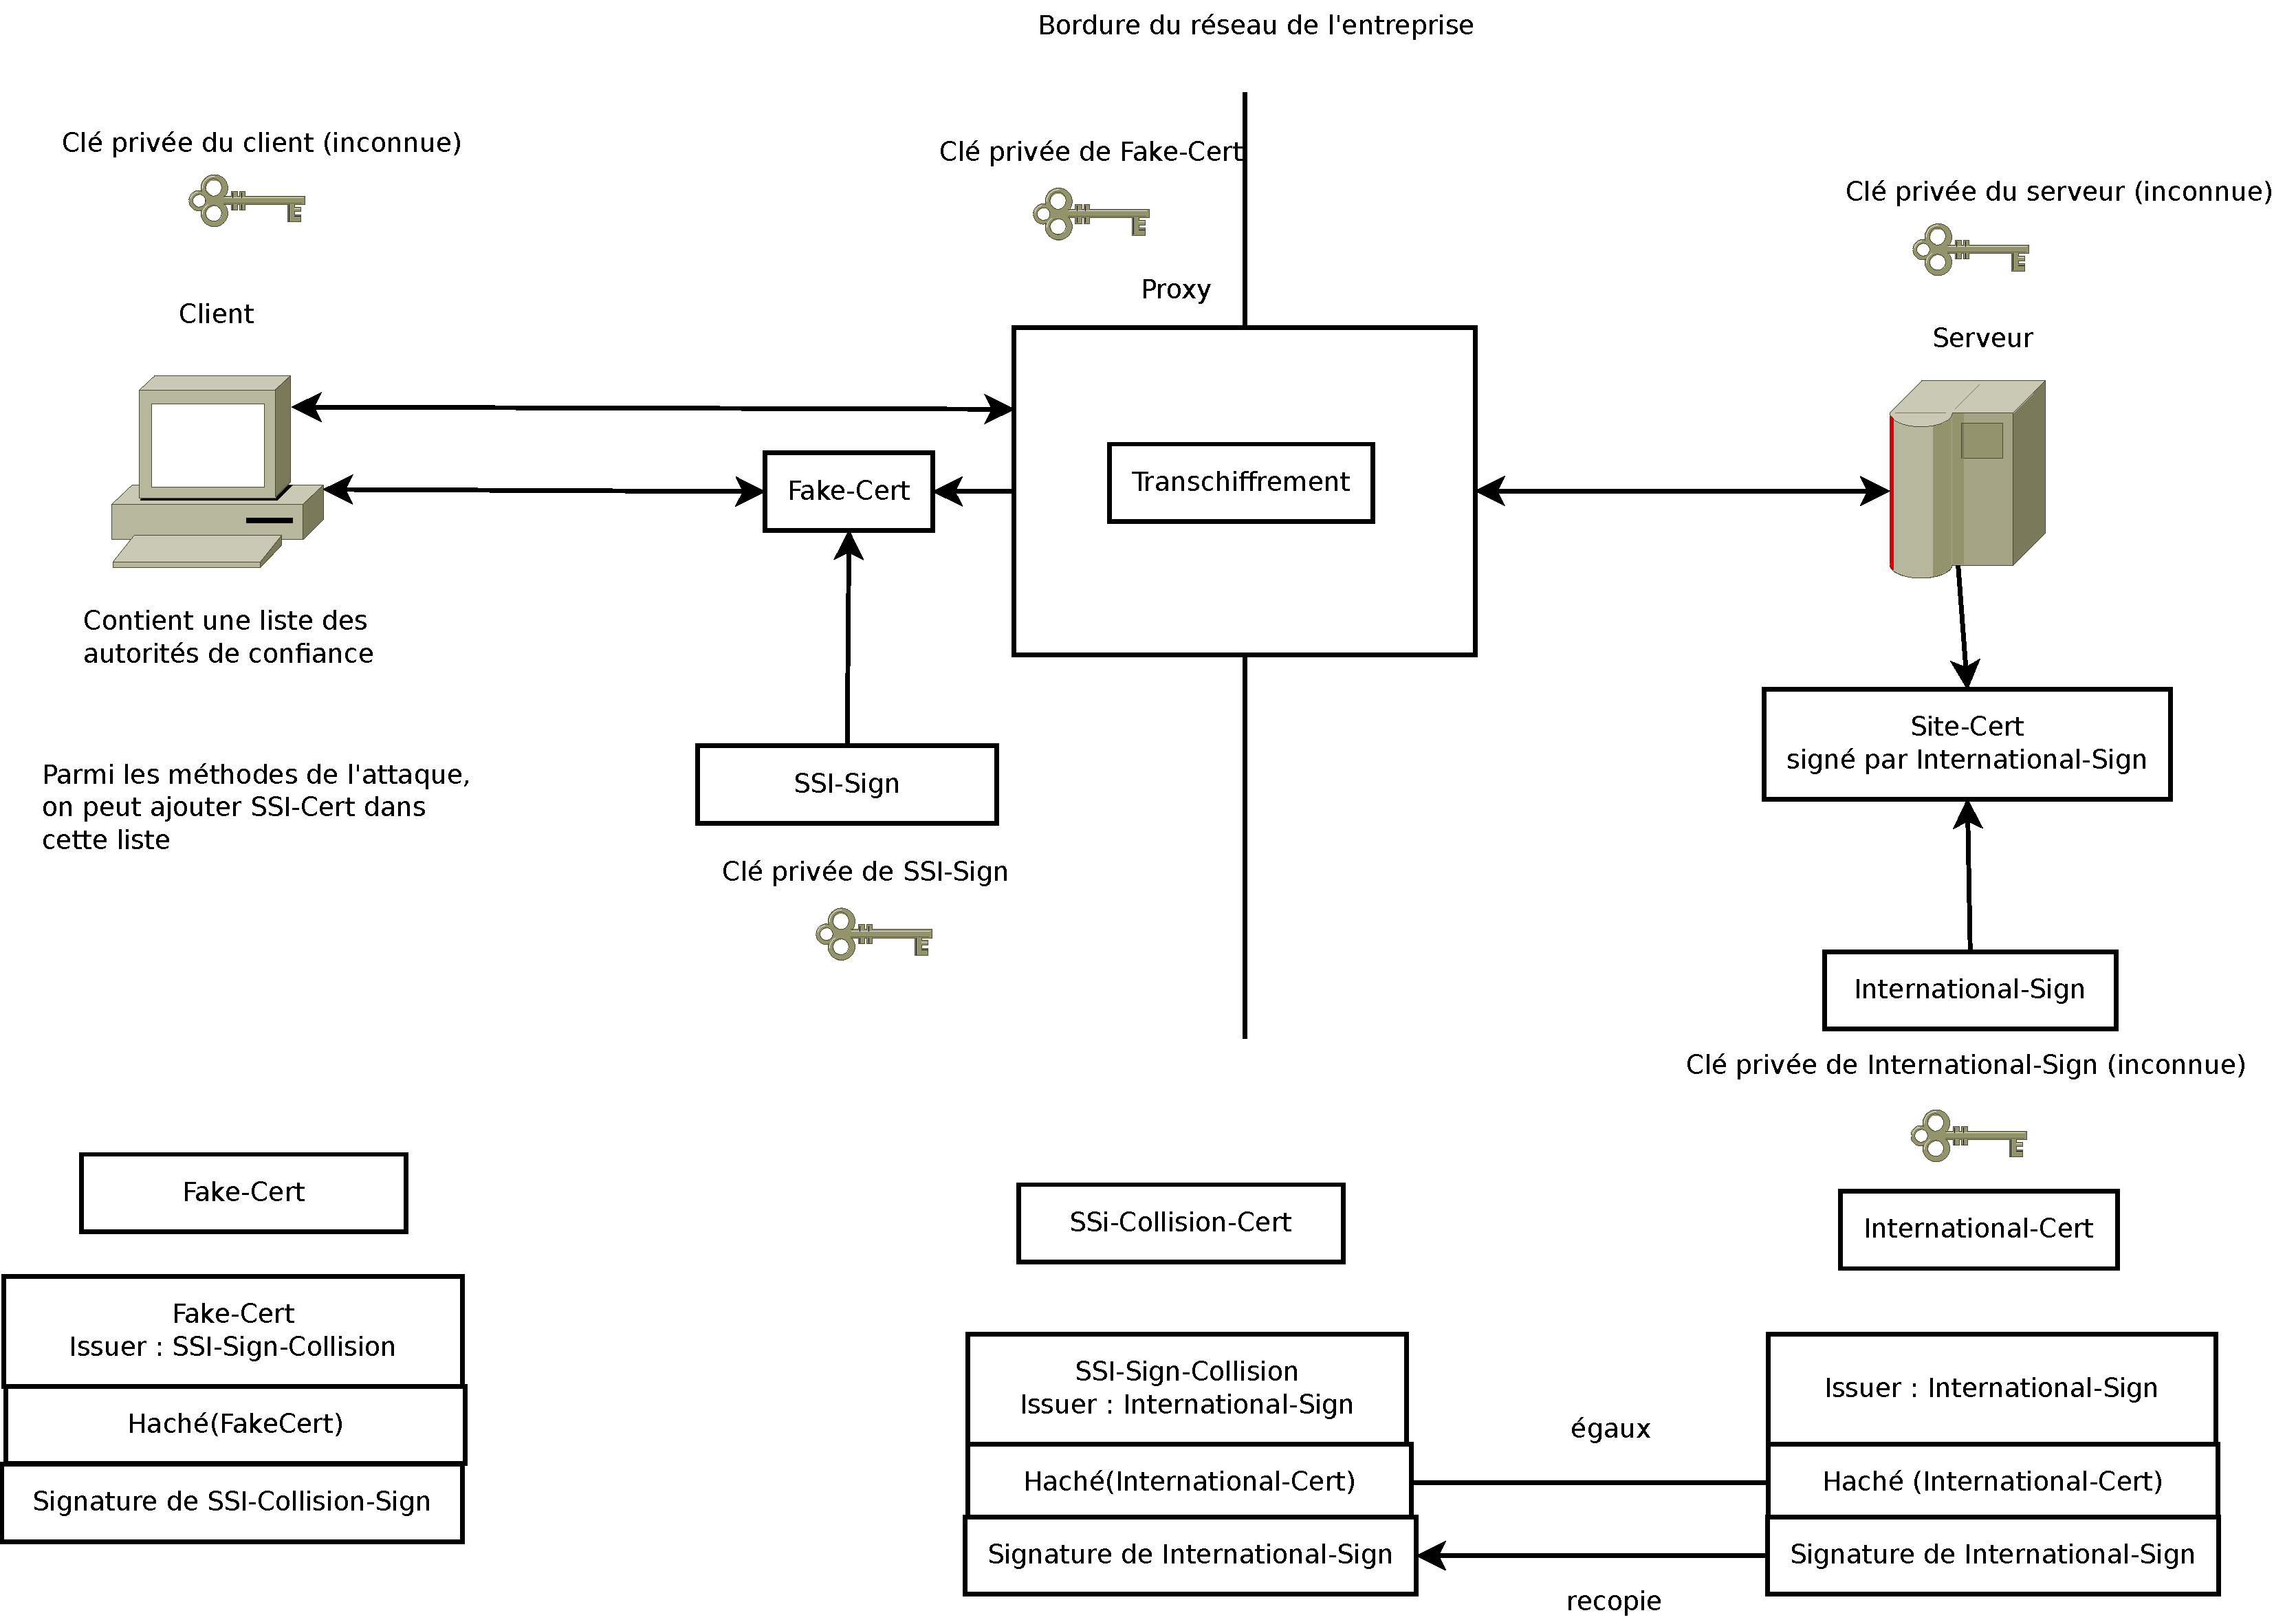
\includegraphics[width=\textwidth]{../STB/images/schema_autorites.pdf}

\end{frame}
